\chapter{Primos}
\label{chap:primos}

No Capítulo \ref{chap:div} vimos as principais ferramentas 
relacionadas aos números primos no \Sage. Nesse capítulo
iremos usar essas e outras ferramentas para explorar propriedades e
resultados importantes sobre primos. Uma referência fundamental para
os aspectos computacionais dos números primos pode
ser vista em \cite{crandall2006prime}
 


\section{Fórmulas que geram?}

\section{Pseudoprimos (Expandir a discussão)}

\subsection{Pseudoprimos de Fermat}


O Pequeno Teorema de Fermat afirma que se $p$ é primo
e $1\leq a<p$, então $a^{p-1}$ deixa resto $1$ na
divisão por $p$. Geralmente esse teorema é apresentado
usando a linguagem de aritmética modular, como veremos
no Capítulo \ref{chap:modular}. 

Podemos usar a contrapositiva desse fato
para concluir que $n$ é composto: basta encontrar  algum $1\leq a< n$
tal que $a^{n-1}$ não deixa resto $1$ na divisão por $n$. A recíproca,
no entanto, não é válida --- existem naturais
$n$ e $1\leq a < n$, tais que $a^{n-1}$ deixa resto
$1$ na divisão por $n$ mas $n$ não é primo. Nesse caso dizemos que
$n$ é pseudoprimo na
base $a$. 

\begin{exercise}
  Usando os métodos \ils{is\_prime} e \ils{quo\_rem}
encontre os $100$ primeiros pseudoprimos de Fermat na base $2$.
\index[sage]{\ils{is\_prime}}
\end{exercise}

\begin{exercise}
  Generalize o seu código do exercício anterior para encontrar
  os $k$ primeiros pseudoprimos de Fermat em uma base $a\geq 2$ 
  arbitrária. (existe um teorema que garante a existência de infinitos
  pseudoprimos de Fermat para qualquer base $a \geq 2$, veja
  \cite[Theorem 3.4.4]{crandall2006prime})
\end{exercise}

\begin{exercise}
  Pesquise sobre números de Carmichael e encontre os $5$ primeiros.
\end{exercise}

Qualquer teorema do tipo ``\emph{se $p$ é primo então $S(p)$}",
onde $S$ é uma afirmação sobre naturais, induz uma noção
de pseudoprimo: Se $n$ é um número composto para
qual a afirmação $S(n)$ é válida, dizemos que $n$ é um
$S$-pseudoprimo. Sendo assim, se a condição $S$ for
fácil de ser verificada, podemos utilizá-la como
um teste de  primalidade probabilístico. Claramente
só nos interessa o caso em que que existem poucos 
$S$-pseudoprimos. Por exemplo, todo primo $p$
satisfaz $S(n)$, onde $S(n)$ é a 
condição \emph{$n$ é igual a $2$ ou é ímpar}, no 
entanto existem muitos pseudoprimos associados a
essa condição com relação aos primos já que
todos os ímpares compostos a satisfazem. 

Dessa forma, teoremas
que indicam a relação entre os pseudoprimos sob
uma condição $S$ e os verdadeiramente primos 
são muito importantes. Há certas propriedades
para as quais não se conhece nenhum pseudoprimo. 
MELHORAR ESSA DISCUSSÃO




\section{Distribuição}

Como discutimos, o estudo do comportamento dos números primos
é um dos principais tópicos de estudo de uma área chamada
Teoria Analítica dos Números. O objeto mais importante
dessa área é, sem dúvida, a função de contagem dos números
primos \index{Função!$\pi$, contagem de primos}
$\pi:\RR_{\geq 0} \to \ZZ_{\geq 0}$ que associa a cada
número real positivo $x$ a quantidade de primos menores
ou iguais a $x$, isto é:
$$
  \pi(x):= \#\{p \in \NN \mid p\text{ primo e } p\leq x\}
$$

Com as funções apresentadas no Capítulo \ref{chap:div}
não deve ser difícil você mesmo criar a sua função $\pi$.
A função $\pi$ implementada no \Sage é chamada de \ils{prime\_pi}.
\index[sage]{\ils{prime\_pi}}
\begin{sageinput}
print("pi(200)\t=", prime_pi(200))
print("pi(6.9)\t=", prime_pi(6.9))
\end{sageinput}
\begin{sageoutput}
pi(200) = 46
pi(6.9) = 3
\end{sageoutput}

Podemos visualizar o gráfico da função $\pi(x)$ através
da ferramenta \ils{plot} do \Sage.
\index[sage]{\ils{plot}}
\begin{sageinput}
plot(prime_pi,10,100)
\end{sageinput}
\begin{figure}[h]
  \centering
  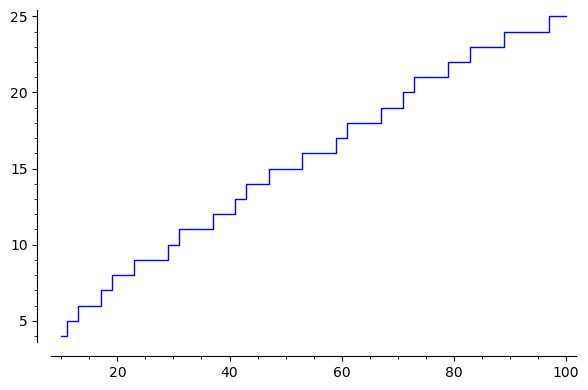
\includegraphics[scale=0.7]{imgs/prime_plot.png}
  \caption{Gráfico de $\pi(x)$}
  \label{img:primeplot}
\end{figure}

Muitos dos resultados sobre o comportamento e a distribuição de primos
são escritos usando a função $\pi(x)$, há um interesse especial em outras
funções reais que aproximam $\pi(x)$. Uma aproximação
em particular, encontrada por Legendre e Gauss e 
provada cerca de um século depois, é tão importante que ganhou
o nome de \emph{Teorema dos Números Primos}.
A hipótese de Riemann 
um dos maiores problemas em aberto na matemática, é equivalente
a certas estimativas sobre o erro na aproximação de $\pi(x)$.
Discutiremos algumas dessas aproximações
mais adiante. Antes disso, vejamos um exemplo mais elementar.
O matemático francês Joseph Bertrand conjecturou em 1845 que
\index{Postulado de Bertrand}
entre um inteiro $n>1$ e seu dobro sempre há um número primo;
isto é, existe um $p$ primo com $n\leq p\leq 2n$. Ora, como
$\pi(2n)$ conta os primos até $2n$ e $\pi(n)$ até $n$,
essa afirmação é equivalente a $\pi(2n)>\pi(n)$, ou seja,
$\pi(2n) - \pi(n) \geq 1$.
Observe na figura \ref{fig:bertrand} o comportamento de
$\pi(2n) - \pi(n)$ para $n$ entre $100$ e $300$.
\begin{sageinput}
def bertrand(n):
    return prime_pi(2*n) - prime_pi(n)
plot(bertrand,100,300,color='black')
\end{sageinput}
\begin{figure}[h]
  \centering
  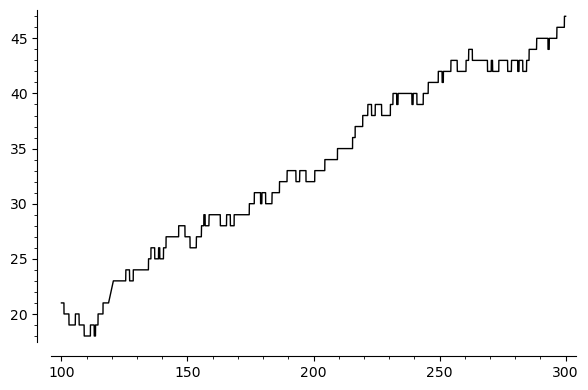
\includegraphics[scale=0.7]{imgs/bertrand.png}
  \caption{$\pi(2n) - \pi(n)$}
  \label{fig:bertrand}
\end{figure}
Observe que, ao contrário de $\pi(n)$, que é naturalmente
não decrescente, ${\pi(2n)-\pi(n)}$ não é monótona. No entanto,
parece ser claro que essa quantidade nunca atinge o valor $1$.
De fato, a conjectura de Bertrand, conhecida como Postulado
de Bertrand, foi demonstrada alguns anos depois pelo matemático
russo Chebyshev. A prova se baseia em estimativas
envolvendo o número binomial ${2n \choose n}$, a suposição
que nenhum primo $p>n$ divide ${2n \choose n}$ implica
em uma cota máxima para $n$. Dessa forma, naturais $n$
maiores que essa cota não satisfazem essa propriedade,
e portanto há um primo $n<p<2n$ e, para naturais menores
que tal cota a afirmação pode ser verificada
computacionalmente, veja \cite[Sec. 5.3]{tnumgugu}.
Diversos outros resultados em teoria dos números são obtidos
de forma similar: prova-se formalmente que o resultado vale 
a partir de determinada constante $K$ e o caso
$n\leq K$ é verificado computacionalmente.
Vale observar que o postulado
de Bertrand pode ser visto como uma consequência direta 
do Teorema dos Números Primos e, como o gráfico 
indica, a quantidade de primos entre $n$ e $2n$
tende a infinito quando $n\to \infty$. 

% teorema dos números primos
\begin{table}
$$
\begin{array}{crrr}
x  & \pi(x) & x/\log(x) & \frac{\pi(x)}{(x/\log(x))} \\ \hline
10  & 4 & 4.34 & 0.92103 \\
10^2  & 25 & 21.71 & 1.15129 \\
10^3  & 168 & 144.76 & 1.16050 \\
10^4  & 1\,229 & 1\,085.74 & 1.13195 \\
10^5  & 9\,592 & 8\,685.89 & 1.10432 \\
10^6  & 78\,498 & 72\,382.41 & 1.08449 \\
10^7  & 664\,579 & 620\,420.69 & 1.07117 \\
10^8  & 5\,761\,455 & 5\,428\,681.02 & 1.06130 \\
10^9  & 50\,847\,534 & 48\,254\,942.43 & 1.05373 \\
10^{10}  & 455\,052\,511 & 434\,294\,481.90 & 1.04780 \\
10^{11}  & 4\,118\,054\,813 & 3\,948\,131\,653.67 & 1.04304 \\
10^{12}  & 37\,607\,912\,018 & 36191\,206\,825.27 & 1.03915 \\
10^{13}  & 346\,065\,536\,839 & 334\,072\,678\,387.12 & 1.03590 \\
\end{array}
$$
\caption{$\pi(x)$, $x/\log(x)$  seu quociente}
\label{tab:tnplog}
\end{table}

$$
  \lim_{x \to \infty}
    \frac{\pi(x)}{\left(\frac{x}{\log x}\right)} = 1
$$

Usamos a notação $\pi(x) \sim \frac{x}{\log x}$

Podemos interpretar o limite acima como a afirmação
que, para $x$ grande, a probabilidade de que um
inteiro menor que $x$ seja primo, isto é, $\pi(x)/x$,
é aproximadamente $1/\log{x}$

\section{Primos em PA}


\section{Funções Aritméticas}
\label{sec:funarit}
 
Chamamos de \emph{função aritmética} uma função da forma
\index{Função!Aritmética}
$f:\NN \to \CC$, nesse texto estudaremos
exclusivamente funções aritméticas cujo contra domínio
é o conjunto dos reais. Gostaríamos que as funções aritméticas 
expressassem propriedades aritméticas sobre os inteiros, para
isso vamos definir mais duas propriedades sobre funções aritméticas:

\begin{itemize}
  \item  Uma função $f:\NN \to \RR$ é dita multiplicativa se
  $f(ab) = f(a)f(b)$ sempre que $a,b \in \NN$ forem coprimos.
  \item  Uma função $f:\NN \to \RR$ é dita completamente
  multiplicativa se $f(ab) = f(a)f(b)$ para quaisquer $a,b \in \NN$.
\index{Função!Multiplicativa}
\end{itemize}

Já introduzimos implicitamente uma importante função
aritmética. Ao discutirmos números perfeitos falamos
sobre a soma dos divisores de um inteiro e usamos a soma
da lista gerada pela 
função \ils{divisors}. Defina \index{Função!Sigma $\sigma$}
$\sigma:\NN \to \RR$ dada por $\sigma(n) =$ soma
dos divisores positivos de $n$. Representamos
matematicamente essa soma por $\sigma(n) = \sum_{d\mid n} d$. Note que
embora não esteja explicito no somatório, somamos apenas os
divisores positivos.

No \sage a função 
$\sigma(n)$ pode ser calculada usando
\ils{sum(divisors(n))}. Como, ao definir números perfeitos,
consideramos apenas os divisores positivos próprios,
isto é, diferentes de $n$, podemos redefinir números
perfeitos como naturais $n$ satisfazendo $\sigma(n) = 2n$.

A função $\sigma$ pode ser generalizada da seguinte forma:
para $k\geq 0$ inteiro, defina $\sigma_k:\NN \to \RR$
por $\sigma_k(n) = \sum_{d\mid n} d^k$, de forma
que $\sigma_1 = \sigma$. 
Se $k=0$ então
$\sigma_0(n) = \sum_{d \mid n} 1 = $ quantidade de divisores
positivos de $n$, essa função também é denotada por $d(n)$ ou
$\tau(n)$ (não confundir com a função $\tau$ de Ramanujan).

\begin{exercise}  \label{ex:sigma}
  Usando a função \ils{divisors}, crie um código
  que calcule $\sigma_k(n)$ para $k$ e $n$ dados. Usando a
  compreensão de listas isso pode ser feito em apenas uma linha.
\end{exercise}  

O \sage já possui as funções $\sigma_k$ implementadas: $\sigma_k(n)$
pode ser calculado com \ils{sigma(n,k)}, sendo o segundo argumento
\index[sage]{\ils{sigma}}
opcional e tomado como $k=1$ se ausente, isto é, \ils{sigma(n)}
irá retornar $\sigma_1(n) = \sigma(n)$\footnote{Se,
ao resolver o exercício acima, você criou uma função com o nome \ils{sigma},
então ela sobrescreveu a do \sage. Para recuperar a função original basta
reiniciar o sage, reiniciando o kernel se estiver executando um notebook.}
. No entanto, o \sage não
calcula o valor de $\sigma_k$ de forma como fizemos no exercício
\ref{ex:sigma} --- para os mais corajoso, digite \ils{sigma??} e 
tente encontrar o pedaço do código onde a função é realmente calculada.
Isso será justificado após o exercício a seguir:

\begin{exercise}
  Crie um código que escolha pares de naturais $a$ e $b$ coprimos
  aleatórios, calcule $\sigma_k(a)$, $\sigma_k(b)$ e $\sigma_k(ab)$ e
  compare $\sigma_k(a)\sigma_k(b)$ com $\sigma_k(ab)$. Após se convencer
  que $\sigma_k$ é multiplicativa prove esse fato. (Dica: Prove primeiramente
  que se $a$ e $b$ são coprimos e $D_n$ representa o conjunto dos divisores
  positivos de $n$, então existe uma bijeção $D_{a}\times D_{b} \to D_{ab}$).
\end{exercise}


Considere agora um natural $n>1$ e uma função multiplicativa $f$. Se
a fatoração em primos de $n$ é dada por $n=p_1^{e_1} \dots p_r^{e_r}$,
então, como $f$ é multiplicativa
$$
  f(n) = f(p_1^{e_1} \cdots p_r^{e_r}) = f(p_1^{e_1}) \cdots f(p_r^{e_r}),
$$
ou seja, $f$ depende apenas do comportamento nas potências de primos.
Assim, para calcular $f(n)$ onde $f$ é uma função multiplicativa, basta
conhecer os valores de $f$ nas potências de primos e a fatoração em primos
de $n$. 

\paragraph{Função $\varphi$ de Euler}
Uma das funções aritméticas mais importantes é a função $\varphi$ de Euler,
definida da seguinte forma:
$$
  \varphi(n) = \#\{1\leq a \leq n \mid \mdc(a,n) = 1\}
$$
\index{Função!$\varphi$ de Euler}
Para uma potência de primo, digamos $p^e$, $\varphi(p^e)$ conta
os coprimos com $p^e$. Como o único divisor primo de $p^e$  é o próprio
$p$, contamos quantos naturais $1\leq a \leq p^e$, não são divisíveis por
$p$. Existem $p^{e-1}$ multiplos de $p$ menores que $p^e$, portanto
$\varphi(p^e) = p^2 - p^{e-1}$. No \sage, a função de Euler é
implementada na função \ils{euler\_phi}. \index[sage]{\ils{euler\_phi}}

\begin{exercise}
Repita a parte inicial do exercício \ref{ex:sigma}. A demonstração da
multiplicatividade de $\varphi$ exige alguns resultados auxiliares.
Voltaremos a discutir essa função no capítulo \ref{chap:modular}.
\end{exercise}

Como mencionamos, uma função aritmética multiplicativa depende
apenas dos seus valores nas potências de primos. Isso permite
criar funções aritméticas multiplicativas de forma simples,
basta definirmos a função em cada potência de primo $p^e$
e, para um $n \in \NN$ qualquer, basta expandir a definição
usando a multiplicatividade. Note, no entanto, que a condição
de multiplicatividade implica $f(a) = f(a\times 1)= f(a)f(1)$,
portanto $f(1) = 1$ ou $f(a) = 0$ para todo $a \in \NN$.

\begin{example}
  Nesse exemplo implementamos a função aritmética multiplicativa dada por
  $\psi(p^e) = p^e + p^{e-1}$ se $e >0$ e $\psi(1) = 1$.
  Primeiramente criamos a função \ils{psi\_pp} para calcular $\psi$ apenas
  nas potências de primos.
\begin{sageinput}
def psi_pp(n):
    fatoracao = factor(n)
    if len(fatoracao) != 1:
        return "Erro: {} nao potencia de primo".format(n)
    p = fatoracao[0][0]
    e = fatoracao[0][1]
    return p^e + p^(e-1)
    
print("psi(16) =", psi_pp(16))
print("psi(22) =", psi_pp(22))
\end{sageinput}
\begin{sageoutput}
psi(16) =  24
psi(22) =  Erro: 22 nao potencia de primo
\end{sageoutput}
A função \ils{psi} abaixo agora calcula o valor de $\psi(n)$ para
qualquer $n$.
\begin{sageinput}
def psi(n):
    if n <= 0:
        return "Erro: n deve ser positivo"
    if n == 1:
        return 1
    fatoracao = factor(n)
    total = prod([psi_pp(p^e) for (p,e) in fatoracao])
    return total

[psi(i) for i in [1..20]]
\end{sageinput}
\begin{sageoutput}
[1, 3, 4, 6, 6, 12, 8, 12, 12, 18, 12, 24, 14, 24, 24, 24, 18, 36, 20, 36]
\end{sageoutput}
A função \ils{psi} que definimos acima é a função $\psi$ de Dedekind
e tem conexões com a teoria de formas modulares\footnote{A função $\psi$
de dedekind também já está implementada no \sage, mas é necessário
importá-la usando \ils{from sage.arith.misc import dedekind\_psi}.
Na verdade, ao chamar nossa função de \ils{psi}
sobrescrevemos uma função já existente no \sage, chamada
função digamma.}.
\end{example}



\begin{exercise}
Listamos a seguir algumas das principais funções aritméticas.
Para cada uma delas crie um código que calcule tais funções em
um $n$ dado, como fizemos com a função $\psi$ acima. Usamos 
a seguinte notação, se $n \in \NN$ e $n = p_1^{e_1} \cdots p_r^{e_r}$
é a sua fatoração em primos, então
$\omega(n) = r$ e $\Omega(n) = e_1+e_2+\cdots+e_n$. 
Conjecture quais dessas funções são (completamente) multiplicativas
ou (completamente) aditivas. Você consegue provar alguma dessas afirmações?
\begin{table}
\centering
{\renewcommand{\arraystretch}{2.4}
  \begin{tabular}{|l|l|} \hline
    Função & Definicao \\ \hline \hline
    $\mu$ de Möbius & $\mu(n) = 
      \begin{cases}
        (-1)^{\omega(n)} & \text{ se } \omega(n) = \Omega(n) \\ 
        0 & \text{ se } \omega(n) \neq \Omega(n) \\
      \end{cases}$ \\ \hline
    $\lambda$ de Liouville & $\lambda(n) = (-1)^{\Omega(n)}$ \\ \hline
    Soma de Ramanujam &
      $c_q(n) = \sum_{\stackrel{1 \leq a \leq q}{\mdc(a,q) = 1}}
          e^{2\pi i \frac{a}{q}n}$ \\ \hline
    Ordem $p$-ádica & $v_p(n) = \max\{k \geq 0 \mid p^k \mid n\}$ \\ \hline
    von Mangoldt  & $\Lambda(n) = 
    \begin{cases}
      \log(p) & \text{ se } n = p^k \\
      0 & \text{ caso contrário }
    \end{cases}$ \\ \hline
  \end{tabular}}
  \caption{Funções Aritméticas}
  \label{tab:funarit}
\end{table}
\end{exercise}



\newpage
\section{Explore!}
\label{sec:exploreprimos}
\subsection{Primos de Mersenne, GIMPS}

\subsection{Mais conjecturas: Opperman}

\begin{itemize}
  \item Primos especiais (de sophie  germain,etc)
\end{itemize}

\section{Exercícios}

\begin{exercise}
  Construa um código \Sage que crie a Tabela \ref{tab:tnplog}.
\end{exercise}

\begin{exercise}
    Seja $n \in \NN$ e considere a sequência $s_k$ de naturais dada por
    $s_0 = n$ e $s_k = \sigma(s_{k-1}) - s_{k-1}$.
    % terminando a sequência se ela chega no $1$, já que
    % a $\sigma(1) = 1$, ou se a sequência se repete, ou seja,
    % se $s_k = s_l$ para algum $l<k$, nesse caso dizemos
    % que a sequência tem comprimento $k$, nesse caso dizemos
    % que a sequência termina em um ciclo de comprimento $k-l$.
    Por exemplo, para $n = 12$,
    $(s_k) = (12,16,15,9,4,3,1,1,1,\dots)$, 
    para $n = 6$, $(s_k) = (6,6,6,\dots)$.
    As sequências $(s_k)$ são chamadas de \emph{sequência de alíquota}
    \index{Sequência!de alíquota}.
    \begin{itemize}
      \item[a)] Crie um código que calcule a sequência de alíquota
      até um índice dado; isto é, o seu programa deve receber
      $n$ e $i$ e retornar $(s_0,s_1,\dots,s_i)$.
      \item[b)] Prove que a sequência é eventualmente
      constante se chega em algum número perfeito.
      \item[c)] Prove que a sequência termina em um
      ciclo de comprimento $2$ se chega em algum número
      amigável.
      \item[d)] Naturais cuja sequência de alíquota são ciclos
      de comprimento maior que $2$ são ditos \emph{sociáveis}. Encontre o menor
      número sociável $n$ cuja sequência de alíquota
      é um ciclo de comprimento $4$. {\color{red}(verificar, talvez demore muito)}
        %Segundo Wikipedia, 1,264,460 
      \index{Número!Sociável}
      \item[e)] Repita o item anterior para um ciclo de comprimento
        {\color{red}(verificar, talvez demore muito)}
        $5$. %Segundo Wikipedia, 12,496 
      \item[f)] Um número é dito intocável
      \index{Número!Intocável} se não está em nenhuma sequência de alíquota,
      exceto a iniciada por ele, ou seja, não é a soma dos divisores próprios
      de nenhum outro natural. Encontre os $5$ primeiros números
      intocáveis.
    \end{itemize}
\end{exercise}


\begin{exercise}
  Dadas duas funções aritméticas $f,g$, definimos o produto ou
  convolução de Dirichlet de $f$ e $g$ como a função aritmética $h$
  dada por 
  $$
    h(n) = \sum_{d \mid n} f(d) g\left(\frac{n}{d}\right)
  $$
  A notação para convolução de Dirichlet é $f*g$.
  \begin{itemize}
    \item[a)] Prove que se $f$ e $g$ são multiplicativas
    então $f*g$ também é multiplicativa.
    \item[b)] Crie um código que calcule a convolução de Dirichlet
    de duas funções aritméticas dadas.
  \end{itemize}
\end{exercise}